\documentclass[12pt]{article}
\usepackage{isolatin1,a4wide,graphicx,SHmathnot,url}
\usepackage{hyperref}

\hypersetup{backref, pdfpagemode=none, colorlinks=true, linkcolor=blue, 
anchorcolor=blue, citecolor=blue, filecolor=blue, menucolor=blue,
pagecolor=blue, urlcolor=blue}% Configuration in the file hyperref.cfg 

\usepackage[authoryear,round,longnamesfirst]{natbib}
%\usepackage{listings}
%\lstset{language=R}

%\usepackage{enumerate,isolatin1}
%\usepackage{epsfig}
%\usepackage{latexsym} 
\usepackage{amsmath, theorem}
%\usepackage[mathscr]{eucal}
%\usepackage{amssymb}       % Sikrer paene \mathbb
%\usepackage{times,graphicx}
\def\sspir{\texttt{sspiR}}
\def\R{\texttt{R}}
\def\ctmm{{\tt C2MM}}
\def\tsp{^\top}
\def\wiki#1{ \href{#1}{[Wikipedia]} }

\title{Overview over Dynamical Statistical Models -- with a view
  towards application in biological sciences} 

\author{S�ren H�jsgaard}


\begin{document}

\maketitle
\tableofcontents
\openup2pt

\section{Introduction}
\label{sec:intro}

This paper is intended to give an overview over some aspects of
dynamical statistical models (hereafter abbreviated DSMs) with a view
towards applications in biological sciences. The specific view we have
is to applications where data are measured online and where interest
is utilizing data as they arrive (as opposed to waiting until a whole
batch of data is available for an analysis). 

To set the scene, we let $y_t$ denote a measurement at time $t$. The
observations available up to ancluding time $t$ is denoted either as
$D_t$ or as $y_{1:t}$. Observations avaliable up to but not including
time $t$ are denoted $D_{<t}$ or $y_{<t}$. In the models we consider
there are unknown parameters, generally denoted by $\theta$.
Following this, we are interested in models in which a new observation
$y_t$ measured at time $t$ can readily be incorporated together with
previous observations $y_{<t}$ to provide an updated estimate of a
quantity of interest to be used in e.g.\ a prediction problems

The approaches to DSMs in the engineering, statistical and biological
communities differ in many respects, but there is a gain to be made by
combining the views.

\section{Example: New Hampshire temperatures}
\label{sec:nhtemp}

The data are recordings of the mean annual temperature in degrees
Fahrenheit in New Haven, Connecticut, from 1912 to 1971.  Data are
available in R. A plot of data is shown in Figure~\ref{fig:nhtemp}.

\begin{figure}[ht]
  \centering
  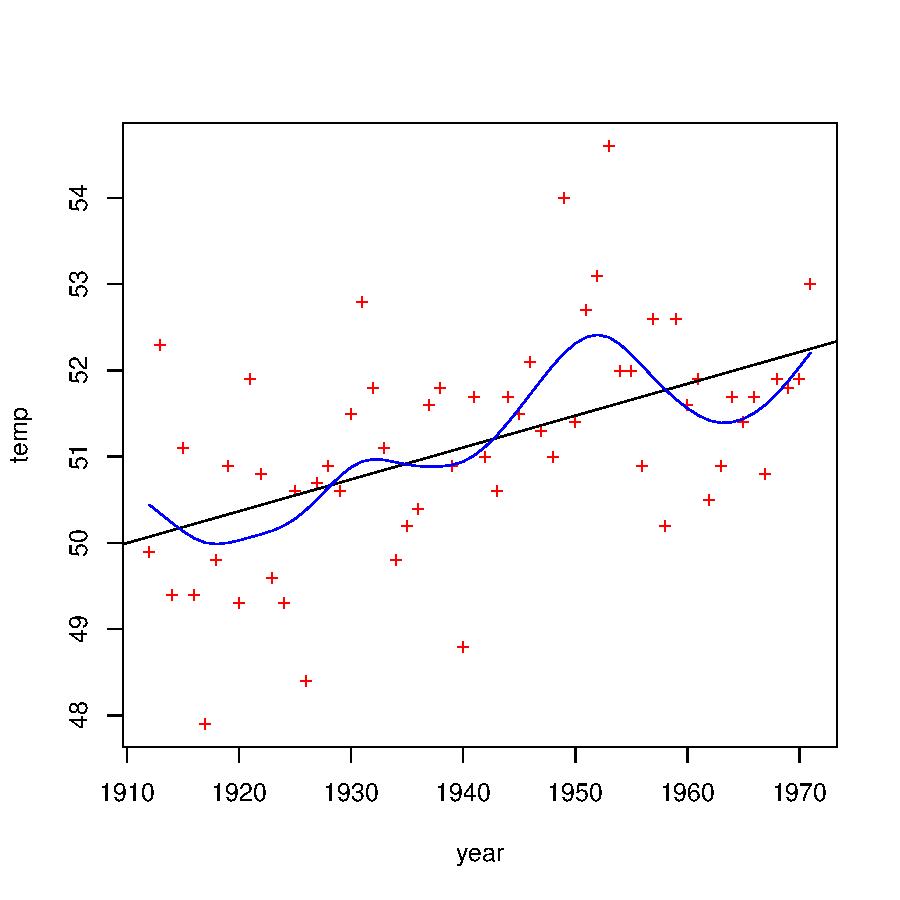
\includegraphics[height=6cm]{fig/nh-002}
  \caption{New Hampshire temperatures  data with linear trend and smoothed spline
    added. }
  \label{fig:nhtemp}
\end{figure}

For simplicity we recode the year as $t=1,2,\dots, 60$. 

\section{Regression and recursive least squares}
\label{sec:reg}

Consider a regression setting model, 
\begin{equation}
  \label{eq:nht-obseq}
  y_t \approx \alpha + \beta t %+ v_t, \ \ \ v_t \sim N(0,\sigma^2_V)  
\end{equation}
%where $v_t$ are the error terms assumed to be independent.  
Suppose the task is to make predictions, and we focus on making 1-step
forecasts. That is given information $D_{t}$ we wish to predict the
temperature in year $t+1$. 

\subsection{Recursive least squares}
\label{sec:xx}

A naive approach is to refit the model to all available observations 
$D_{t}$ every time a new measurement $y_t$ is made. Let
$\theta=(\alpha,\beta)$ and let $\hat\theta_t$ denote the estimate of
$\theta$ based on data $D_t$. Thus $\hat\theta$ is obtained by
minimizing the sum--of--squares,
\begin{equation}
  \label{eq:ss1}
  SS = \sum_{t'=1}^t (y_{t'} - (\alpha + \beta t'))^2.
\end{equation}

In a naive implementation of this approach we will have to store all
data, which might be a problem in some applications. However it is
possible (and in linear models it is quite simple) to avoid this:
Instead we can find $\hat\theta_t$ from $\hat\theta_{t-1}$ and
$(y_t,t)$. This is called \emph{recursive least squares} method. 

\subsection{Recursive least squares with forgetting factor}
\label{sec:xx}


Note that with this method is that observations are ``weighted
equally'' in (\ref{eq:ss1}); that is observations made in the far past
are given the same weight as recent observations. This may not be
appropriate. A very practical alternative is instead to minimize a
weighted sum--of--squares,
\begin{equation}
  \label{eq:ss2}
  SS = \sum_{t'=1}^t \kappa^{t-t'}(y_{t'} - (\alpha + \beta t'))^2.
\end{equation}
for some constant $\kappa$ where $0<\kappa\le 1$. This constant
sometimes called a \emph{forgetting factor} as it describes ``how fast
the past is forgotten'' (down weighted) in the regression. Small
values of $\kappa$ means that the past is forgotten quickly. It is
worth noticing that $\kappa$ can not be estimated directly as part of
a least squares procedure (letting $\kappa$ go to zero means that $SS$
goes to zero no matter the choice of $\theta$). However, on can
estimate $\kappa$ along these lines: Suppose a batch of data is
available.  Let $\hat y_{t+1} =\hat\alpha_t +
\hat\beta_t(t+1)$ be the 1--step prediction of $y_{t+1}$. Note that 
$\hat y_{t+1}$ depends on $\theta,\kappa$ so we might write 
$\hat y_{t+1}=\hat y_{t+1}(\theta,\kappa)$. 
Then the
squared prediction error $(y_{t+1}-\hat y_{t+1}(\theta,\kappa))^2$ is a function of
$(\theta,\kappa)$. We can then estimate $(\theta,\kappa)$ by
minimizing (the non--linear) function:
\begin{equation}
  \label{eq:ss3}
  SS = \sum_{t'=2}^t (y_{t+1} - \hat y_{t+1}(\theta,\kappa))^2.
\end{equation}

Based on this we can obtain an estimate $\hat\kappa$ which can be used
in the dynamic update in (\ref{eq:ss2}). To some people this approach
may appear too much \emph{ad hoc} while other find it perfectly
acceptable. 

See \wiki{http://en.wikipedia.org/wiki/Recursive_least_squares_filter}
for a details and references.


\section{Exponential smoothing and the Holt--Winters filter}
\label{sec:eshw}

In this section we discuss exponential smoothing and the Holt--Winters
filter. 

\subsection{Exponential smoothing}
\label{sec:xx}

Suppose there is no obvious trend in data (which does not apply to the New
Hampshire temperature data), such that data can be
described as ``level + noise''. A \emph{one sided exponential smoothing}
is obtained as
\begin{equation}
  \label{eq:ee1}
  \alpha_t = \kappa y_t + (1-\kappa) \alpha_{t-1} \mbox{ with } \alpha_1 = y_1
\end{equation}
for some constant $\kappa$ where $0<\kappa\le 1$. The 1--step ahead
prediction is then simply $\hat \alpha{t+1} = \alpha_t$. It is illustrative to
write (\ref{eq:ee1}) as
\begin{equation}
  \label{eq:xx}
    \alpha_t = \alpha_{t-1} + \kappa (y_t - \hat \alpha_t ) \mbox{ with } \alpha_1 = y_1
\end{equation}
where $(y_t - \hat \alpha_t )$ can be regarded as the 1--step
prediction error. Note that (\ref{eq:ee1}) has the property that data
are incorporated as they arrive. That is, once $\alpha_{t-1}$ is
calculated there is no need to store $y_t$ (or any of the preceeding
values for that matter). (The term exponential comes from the fact
that observations from the past are downweight at an exponential
rate.) Clearly, $\kappa$ can not be estimated by minimizing the
sum--of--squares, $\sum_t (y_t-\alpha_t)$ because that sum is zero if
$\kappa$ is zero. The parameter $\kappa$ can instead be estimated by
minimizing the 1--step prediction error, i.e.\ by minimizing $\sum_t
(y_t- \hat\alpha_t)^2$ where $\hat\alpha_t$ is the 1--step prediction
based on data up to time $t-1$. 

See \cite{brockwell96its} and \wiki{http://en.wikipedia.org/wiki/Exponential_smoothing}
for a details and references.

\subsection{Holt--Winters filter}
\label{sec:xxx}


If instead there is a (linear) trend in data (as seems to be the case
for the New Hampshire data), an alternative is the Holt--Winters
filter. (This filter applies to other situations as well, but we shall
here focus on the linear case). 

Consider a situation where we have data $D_t$ and wish to make
prediction at time $t+h$. 
The Holt--Winters filter does so as:
\begin{equation}
  \label{eq:hw1}
  \hat y_{t+h} = \alpha_t + \beta_t h
\end{equation}
The parameters $\alpha$ and $\beta$ are updated as
\begin{eqnarray}
  \alpha_t &=& \kappa y_t + (1-\kappa) (\alpha_{t-1} +
  \beta_{t-1})   \label{eq:hw2}  \\
  \beta_t  &=& \delta (\alpha_t - \alpha_{t-1}) + (1-\delta)(\beta_{t-1})
  \label{eq:hw3}
\end{eqnarray}

Hence there are now two smoothing parameters/forgetting factors,
namely $\kappa$ and $\delta$. Note that
setting $\delta=0$ implies that (\ref{eq:hw2}) reduces to
(\ref{eq:ee1}). 

The smoothing parameters are usually estimated from a batch
of data based on minimizing the 1--step prediction error. 

See \cite{winters1960fse} and  
\cite{brockwell96its}
for details and references.


%% 
% and then
% calculate the prediction $\lambda_{t+1} = \alpha + \beta (t+1)$. We can now
% compare $\lambda_{t+1}$ with the actual observation $y_{t+1}$. (Note: Care must
% be taken in the beginning as we need at least data for 3 years to make
% a fit of the line.) The mean squared prediction
% error is 1.5.

% Suppose that interest is also  in prediction  five
% years ahead. Then we can do as before and make predictions 
% $\lambda_{t+5} = \alpha + \beta (t+5)$. 
% Then we obtain the plot in Figure~\ref{fig:nht05}.
% The mean squared prediction
% error is 2.3.

% \begin{figure}[ht]
%   \centering
%   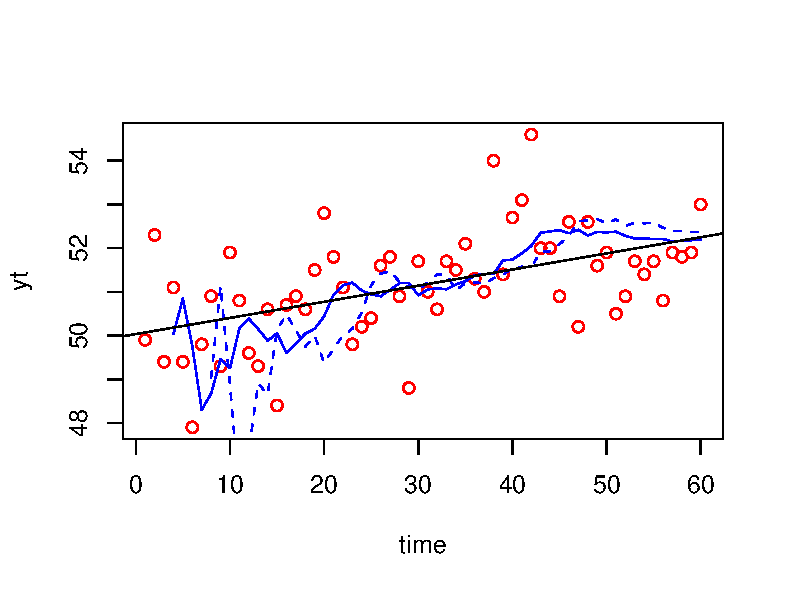
\includegraphics[height=6cm]{fig/nht-05}
%   \caption{New Hampshire temperatures and 1--step (solid line) and
%     5--step (dashed line) predictions based on
%     succesively fitting linear models to data. }
%   \label{fig:nht05}
% \end{figure}


\section{Dynamic linear models}
\label{sec:dlm}



An alternative is to think as follows: Instead of regarding
$(\alpha,\beta)$ as fixed but unknown parameters (who must then
necessarily remain unchanged over time), we allow $(\alpha,\beta)$ to
vary over time.  In particular the slope $\beta$
describes the rate of change in temperature and one could imagine that
this rate would vary (presumably slowly) over time. Hence we imagine that at time $t$
there is a specific value of the parameters $(\alpha_t, \beta_t)$
which we shall also write as $(\alpha,\beta)_t$. Hence we imagine that
$(\alpha,\beta)_t$ varies (slowly) over time. One way of achievieng
this is by postulating that 
\begin{equation}
  \label{eq:nht-syseq}
(\alpha,\beta)_t = (\alpha,\beta)_{t-1} + w_t  
\end{equation}
where $w_t \sim N_2(0,\Sigma_W)$ is a 2--dimensional error
term. 

To
make this work, we must know something about
$(\alpha,\beta)_{0}$, i.e.\ at time zero, i.e.\ before information
starts to arrive. A simple approach is to pick some (sensible)
starting values and write that 
$
(\alpha,\beta)_{0}= m_0 = (m_0^\alpha, m_0^\beta)=(50,0),
$ say. 
However, in practice there is a an uncertainty about
$(\alpha,\beta)_{0}$, so ysually, one would specify a distribution,
\begin{equation}
  \label{eq:nht-prior}
  (\alpha,\beta)_{0} \sim N_2(m_0, C_0)  
\end{equation}

Note two special cases: If $C_0=0$, then we are back to the simple
approach, of simply fixing $(\alpha,\beta)_{0}$ at a specified value. 
If $\Sigma_W=0$, then we are back to the original setting
where $(\alpha,\beta)_t$ is the same at all time points (almost, but
that is subtle little difference). 

The equations \eqref{eq:nht-obseq}, \eqref{eq:nht-syseq} and
\eqref{eq:nht-prior} all together specify a state space model as a
general term. A more specific term is a dynamic linear model (DLM)
because it is essentially a linear model with the additional twist
that the parameters are allowed to vary over time too.


\section{To be random or not to be random}

In a 'classical' regression setting as described in
Section~\ref{sec:nhtemp} the parameters $(\alpha,\beta)$ are regarded
as the true but unknown values. These are estimated, e.g.\ by least
squares regression. 

In Section~\ref{sec:dlm} the situation is different: Consider
\eqref{eq:nht-syseq}. Even if $(\alpha,\beta)_0$ is a fixed quantity,
then $(\alpha,\beta)_1$ will be a random variable because $w_1$ is a
random variable. A random variable is, by definition, random (!) so it
does not make sense to try to estimate it. Instead we estimate some
quantities which describes its distribution, and  a natural choice in
this connection could be the mean and variance. 










\section{Fitting the DLM}

We fit the DLM for the New Hampshire temperatures using the Kalman
filter. The 1--step and 5--step forecasts are displayed in
Figure~\ref{fig:nht06}. The mean squared prediction errors are
respectively 1.4 and 1.6. We have held the variance parameters fixed
at $\sigma^2_V=1$, $\sigma^2_W=\sigma^2_C=0.0001$. 
 
\begin{figure}[ht]
  \centering
  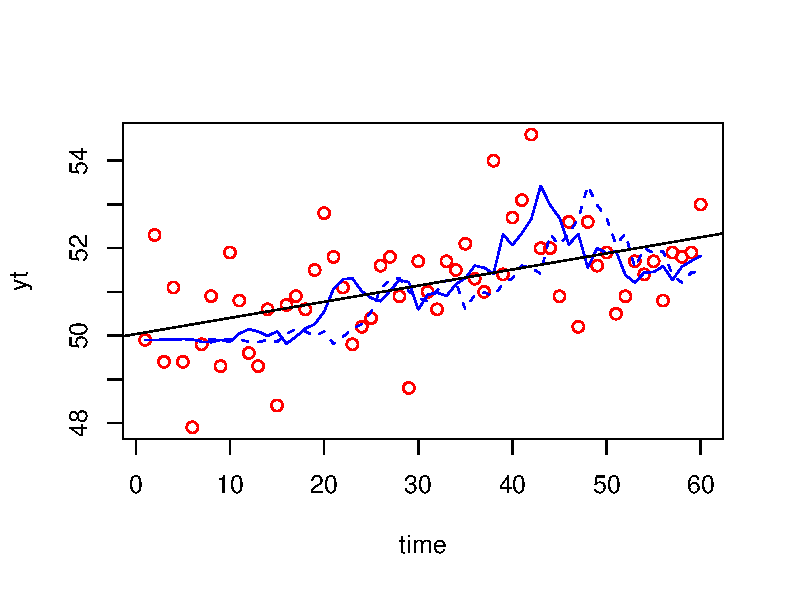
\includegraphics[height=6cm]{fig/nht-06}
  \caption{New Hampshire temperatures and 1--step (solid line) and
    5--step (dashed line) predictions based on fitting the DLM to  data. }
  \label{fig:nht06}
\end{figure}

The Kalman filter is very easy to implement in practice, see
Section~\ref{sec:KFimplement}. 

It is illustrative to look at e.g.\ the degree of smoothing for
different values of the variance parameters. In
Figure~\ref{fig:nht07}, we have fixed $\sigma^2_C=0.0001$ and vary 
$\sigma^2_V$ and $\sigma^2_W$. Smaller values of $\sigma^2_V$ and
larger values of $\sigma^2_W$ leads to
less smooth curves. 

\begin{figure}[ht]
  \centering
  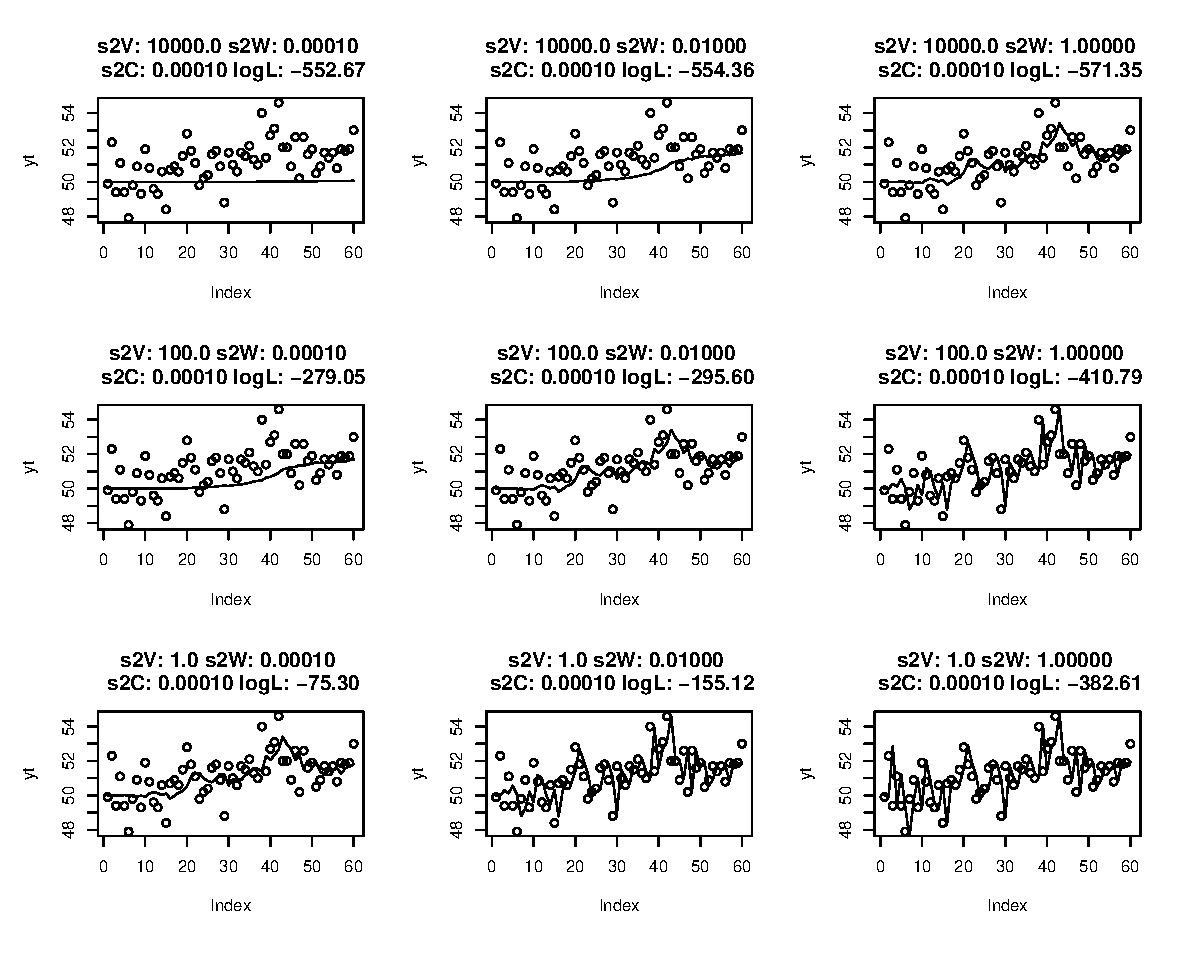
\includegraphics[height=9cm]{fig/nht-07}
  \caption{New Hampshire temperatures and 1--step  
    predictions based on fitting the DLM to data for different values
    of  $\sigma^2_V$ and $\sigma^2_W$. }
  \label{fig:nht07}
\end{figure}


\section{Another state space model}

Consider the model \eqref{eq:nht-obseq} again. If we let $E(y_t)=\mu_t=\alpha +
\beta t$ we get that $E(y_{t+1})= \mu_{t+1} = \mu_t + \beta$,
$E(y_{t+2})= \mu_{t+2} = \mu_t + 2\beta$ and so on. The stochastic
version of this is
\begin{eqnarray}
  y_t &=& \mu_t + v_t\\
  (\mu,\beta)_t &=& (\mu+\beta,\beta)_{t-1} + w_t
\end{eqnarray}



\begin{figure}[ht]
  \centering
  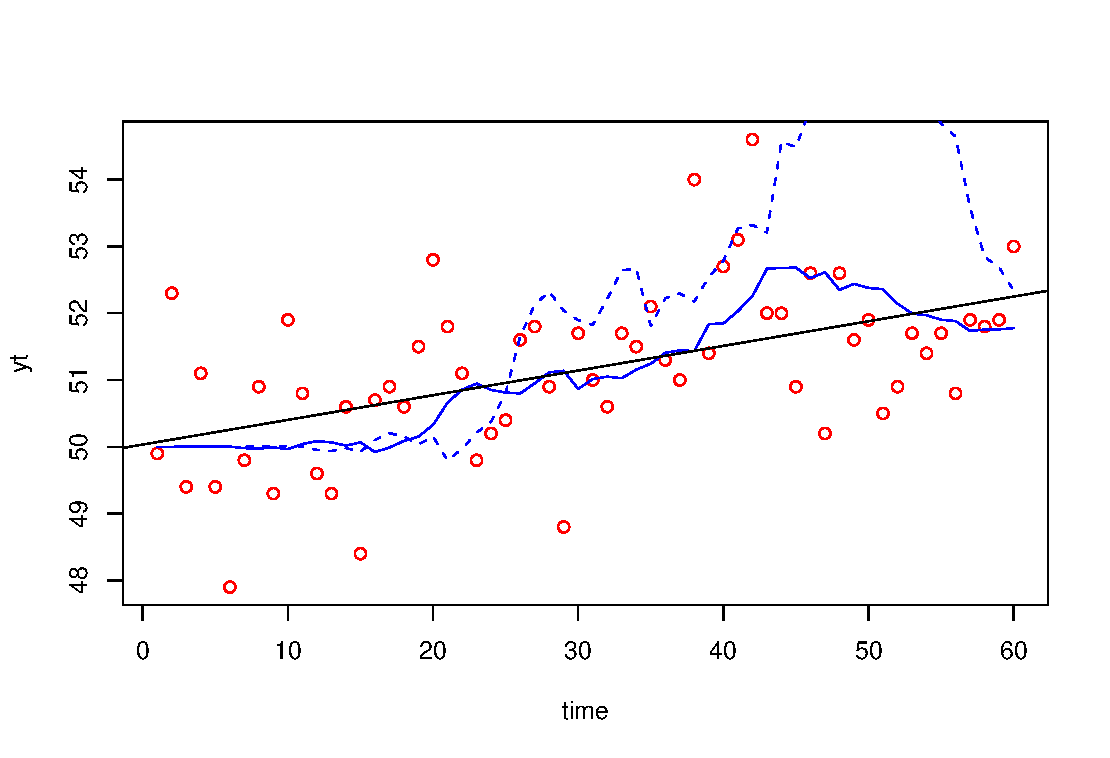
\includegraphics[height=6cm]{fig/nht-09}
  \caption{New Hampshire temperatures and 1--step  
    predictions based after ML estimation of $\sigma^2_V$ and
    $\sigma^2_W$ for three different values of $\sigma^2_C$. }
  \label{fig:nht09}
\end{figure}



Figure~\ref{fig:nht08} shows the result after fitting estimating 
 $\sigma^2_V$ and $\sigma^2_W$ for different values of
 $\sigma^2_C$. (It is in fact also possible to estimate $\sigma^2_C$
 but we abstain from this here). The influence of the prior variance
$\sigma^2_C$ is (not surprisingly) largest at the beginning of the
period.  

\begin{figure}[ht]
  \centering
  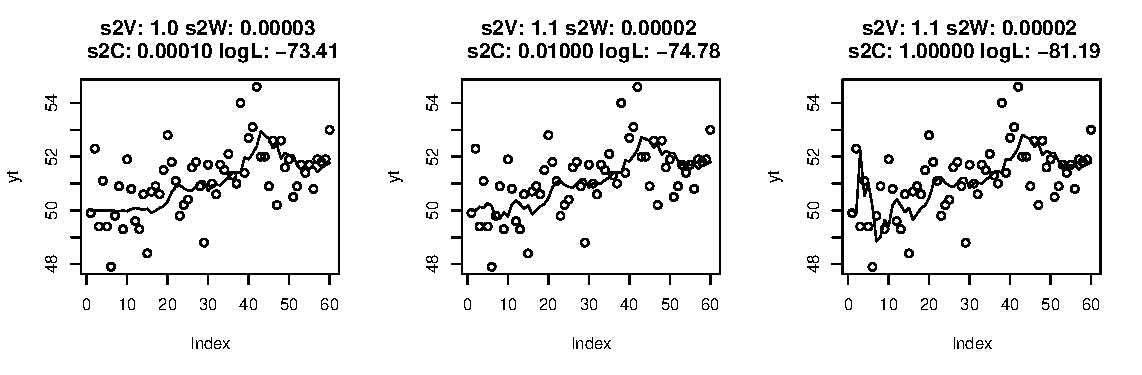
\includegraphics[width=13cm]{fig/nht-08}
  \caption{New Hampshire temperatures and 1--step  
    predictions based after ML estimation of $\sigma^2_V$ and
    $\sigma^2_W$ for three different values of $\sigma^2_C$. }
  \label{fig:nht08}
\end{figure}




\section{State space models}

Linear state space models (SSMs) are traditionally specified as consisting of 
\begin{eqnarray}
y_t &=& F^\top_t \theta_t + v_t, \ \ v_t \sim N(0,V_t)  \\
\theta_t &=& G_t \theta_{t-1} + w_t, \ \ w_t \sim N(0, W_t)\\
\theta_0 &\sim& N(m_0,C_0)
\label{eq:ssm1}
\end{eqnarray}
known as respectively  {\em
  observation equation},
the {\em system equation}
and the 
{\em initial distribution} (of $\theta_0$).
The term $\lambda_t =F_t^\top \theta_t = \EE(y_t|\theta_t)$ is the
{\em signal}.
Thus, technically the 6--tuple $(F_t,V_t,G_t,W_t,m_0,C_0)$ defines a
linear state space model. 

The state space model is a \emph{probabilistic model} for all
$\theta_t$s and all $y_t$s.  An alternative (but equivalent)
formulation is
$$
p(y,\theta) = p(\theta_0) \prod_t p(\theta_t|\theta_{t-1}) p(y_t|\theta_t)
$$
where
\begin{eqnarray}
  \label{eq:dd}
  p(\theta_t|\theta_{t-1}) &:& N(G_t\theta_{t-1}, W_t), 
  %\ \ G_t\theta_{t-1} + w_t, \ \   w_t \sim N(0, W_t)
  \\
  p(y_t|\theta_t) &:& 
  N(F_t^\top \theta_t, V_t), 
  %\ \  F_t^\top \theta_t + v_t, \ \ v_t \sim N(0,V_t) 
\end{eqnarray}


\subsection{Examples of SSMs}
\label{sec:xxx}

Many classical statistical models can be formulated as an
SSM. Consider an autoregression of order 1, i.e.
\begin{equation}
  \label{eq:ar1}
  y_t = \kappa y_{t-1} + v_t
\end{equation}
This model can be put in state space form as
\begin{eqnarray}
  y_t &=& \alpha_t \label{eq:ar2}\\
  \alpha_t &=& \kappa \alpha_{t-1} + v_t \label{eq:ar3}
\end{eqnarray}


\section{The Kalman filter}
\label{sec:kfoverview}

Based on observed data we can then calculate  (the distribution of)
the parameters $\theta_t$. 
The Kalman filter (named after its inventor, Rudolf Kalman) is, roughly speaking,
an efficient algorithm for recursively estimating $\theta_t$ when new
observations become available.
The filter was developed in papers by
\cite{kalman:60} and \cite{kalman:61}.  

A wide variety of Kalman filters have now been developed, from Kalman's original
formulation, now called the simple Kalman filter, to the extended
Kalman filter,
the information filter, a variety of square-root filters, unscented
filter, particle filters.

See
\wiki{http://en.wikipedia.org/wiki/Kalman_filter} for an overview and
references. 

The Kalman filter works by ``updating $\theta_t$ as new observations
arrive'', i.e.\ for $t=1, \dots, T$: Given is that
$\theta_{t-1}|D_{t-1}\sim N(m_{t-1}, C_{t-1})$. Then
\begin{eqnarray}
\theta_t | D_{t-1} &\sim& 
N(
\overbrace{G_t,m_{t-p}}^{a_t}, 
\overbrace{G_t C_{t-1}G_t^\top + W_t}^{R_t}
) \\
y_t|D_{t-1} &\sim&
N(
\overbrace{F_t^\top a_t}^{f_t},
\overbrace{F_t^\top R_t F_t + V_t}^{Q_t}
) \\
\theta_t|D_{t} &\sim&
N(
\overbrace{a_t+ \underbrace{R_t F_t
    Q_t^{-1}}_{A_t}\underbrace{(y_t-f_t)}_{e_t}}^{m_t},
\overbrace{R_t - A_t Q_t A_t^\top}^{C_t}
) \label{eq:kf3}
\end{eqnarray}

Hence, the only thing needed to be stored from time $t-1$ to time $t$
is $(m_{t-1}, C_{t-1})$. 
Here $f_t$ is the {1--step forecast}, $e_t$ is the {\em 1--step forecast
  error} while $A_t$ is the {\em Kalman gain}.
%The signal $\lambda_t$ is given $D_{t-1}$  estimated by
%$f_t$. 



For the normal distribution an alternative formulation is as follows:
Since $y_t =F_t^\top \theta_t + v_t$ we have $\cov(y_t,\theta_t)= F_t
\var(\theta_t)$ and so $\cov(y_t,\theta_t|D_{t-1})= F_t^\top
R_t$. 
Hence 
\begin{equation}
  \label{eq:xxx}
  \left(
  \begin{array}{c}
    y_t \\ \theta_t
  \end{array}
  | D_{t-1}
  \right) 
  \sim N
  \left(
    \left[
      \begin{array}{c}
        f_t \\ a_t
      \end{array}
    \right]
    \left[
      \begin{array}{cc}
        Q_t & F_t^\top R_t \\ R_t F_t & R_t
      \end{array}
    \right]
  \right) 
\end{equation}






\subsection{The likelihood}
\label{sec:xxx}

The state space model depends on unknown parameters through $V_t$ and
$W_t$. There are several ways of estimating these; a brute force
approach is the following: We have 
$$
p(y)=\prod_t p(y_t|y_{t-1}, \dots, y_1) = \prod_t p(y_t|D_{t-1})
$$
We have $y_t|D_{t-1}\sim N(f_t,Q_t)$ so 
the log likelihood
$\log L_t$ for a single observation is
$$
\log L_t = -\frac d 2 \log (2\pi) - \frac 1 2 (det(Q_t)+ e_t^\top Q_t^{-1} e_t) 
$$
because
$
L_t = (2\pi)^{-d/2} det(Q_t)^{-1/2} \exp (-\frac 1 2 e_t^\top Q_t^{-1} e_t).
$
Hence the entire log likelihood is 
$$
\log L = -n \frac d 2 \log (2\pi)- \frac 1 2  \sum_t (det(Q_t) + e_t^\top Q_t^{-1} e_t)
$$

This likelihood can be maximized numerically, but it is often not
entirely trivial to get this to work in specific applications. 

\subsection{Online outlier detection}
\label{sec:xxx}

Suppose $y_t$ is $p$ dimensional. Based on $D_{t-1}$ the distribution of
$y_t$ is
$
y_t|D_{t-1} \sim N(f_t, Q_t)
$
so the prediction error is
$$
e_t = y_t-f_t \sim N(0, Q_t)
$$

That means that when $y_t$ is observed but before we update the
equations, we can see how ``likely'' $y_t$ is by noticing
$$
ssd_t = e_t' (Q_t)^{-1} e_t \sim \chi^2_p
$$

This provides a tool for on--line detection of outliers: A large value
of $ssd_t$ suggests that $y_t$ is an ``unlikely observation'', that
is, it might be erroneous. 

\section{Connecting exponential smoothing and state space models}
\label{sec:connect}

There is a close connection between exponential smoothing and
SSMs. Consider exponential smoothing as set out in
Section~\ref{sec:eshw} with
\begin{equation}
  \label{eq:con1}
    \alpha_t = \alpha_{t-1} + \kappa (y_t - \hat \alpha_t ) \mbox{ with } \alpha_1 = y_1
\end{equation}

We can think of $e_t=(y_t - \hat \alpha_t )$ as a prediction error
(which initially is zero). It
is then trivially true that $y_t= \alpha_{t-1}+(y_t- \alpha_{t-1}) =
\alpha_{t-1} + e_t$. Combining this with (\ref{eq:con1}) gives
\begin{eqnarray}
  y_t &=& \alpha_{t-1} + e_t \label{eq:con2}\\
  \alpha_t &=& \alpha_{t-1} + \kappa e_t \label{eq:con3}
\end{eqnarray}
which has a resemblence with the general for of a linear
state space model in (\ref{eq:ssm1}). There are however two important
differences: The error term $e_t$ appears both in the observation and
system equation and there has been made no assumption about the
distribution of the error term. If we assume the error terms to be
normal and independent, then we are almost at (\ref{eq:ssm1}). The
fact that the error term appears in both the observation and system
equation only changes the filter equations slightly; the Kalman filter
can still be used. 

This can be put in a more general setting: Let 
\begin{eqnarray}
  \label{eq:con4}
  y_t &=& F^\top_t \theta_{t-1} + e_t, \ \ e_t \sim N(0,V_t)  \\
  \theta_t &=& G_t \theta_{t-1} + \kappa e_t 
\end{eqnarray}
where $\kappa$ now is a vector in which each element is in
$[0;1]$. From this we find that 
\begin{eqnarray}
  \label{eq:con4}
  y_t &=& F^\top_t \theta_{t-1} + e_t, \ \ e_t \sim N(0,V_t)  \\
  \theta_t &=& G_t \theta_{t-1} + \kappa (y_t- F^\top_t \theta_{t-1}) 
  = D \theta_{t-1} + \kappa y_t,
\end{eqnarray}
say. So $\theta_t$ is hence a weighted sum of $\theta_{t-1}$ and
$t_t$. 

\section{Discussion}
\label{sec:comments}

Purists would often feel uncomfortable with the methods set out in
Sections~\ref{sec:reg} and \ref{sec:eshw}. They are not per se based
on an assumption of an underlying statistical model. We can obtain
parameter estimates, but the way the are obtained appears quite ad hoc
and hence we do not know ``how good they are''.  We can make
predictions, but we do not know how good they are either. On the other
hand, the methods are quite easy to work with in practice and are also
easily implemented. 

The state space models on the other hand appear attractive to some
people because they are based on a proper statistical model, the
parameter estimates have well understood interpretations
(for example, (\ref{eq:kf3}) gives the conditional distribution of $\theta_t$
given $D_t$), the distribution of the prediction errors is known
etc. In practice however, it is usually tricky to estimate the unknown
parameters and therefore one often ends up by stipulating reasonable
values. 

With a view towards biology there are some additional reservations to
be made. In physical/engineering applications there are often (but
certainly not always) differential equations etc.\ which describe a
natural form of the system equation. For example that $d\theta/dt =
h(\theta,t)$ which can be translated into the approximation that
$\theta_t \approx \theta_{t-1} + h(\theta_{t-1}, t-1)$ which yields
the system equation. In biological sciences such quantitative
descriptions are more rare. Therefore, it is often necessary to
stipulate a system equation which essentially provides a smoothing of
the state vector. It is in some cases therefore not clear whether it
is worthwhile to invoke the entire ``Kalman machinery'' for that
purpose (other simpler methods exist for that). 

\section{Acknowledgements}

This work has been carried out in connection with the ILSORM project
which is partly funded by The Danish National Advanced-Technology
Foundation.  




\bibliographystyle{plainnat} \bibliography{fulldef,stat}

\end{document}
\appendix


\section{Conditioning in the MVN distribution}
\label{sec:xxx}


Suppose 
$$
\theta\sim N(a,R), \ \ \ y=F'\theta+v, \ \ \ v\sim N(0,V).
$$ 

Then
$$
\EE(y)=F'a=f, \ \ \ \var(y)=F'RF+V=Q, \ \ \ \cov(y,\theta)=FR.
$$ 

Moreover, 
$(y,\theta)'$ is MVN as
\begin{equation}
  \label{eq:xxx}
  \left(
  \begin{array}{c}
    y \\ \theta
  \end{array}
  \right) 
  \sim N
  \left(
    \left[
      \begin{array}{c}
        f \\ a
      \end{array}
    \right]
    \left[
      \begin{array}{cc}
        F'RF+V=Q & F' R \\ R F & R
      \end{array}
    \right]
  \right) 
\end{equation}

So then 
\begin{eqnarray}
  \label{eq:dd}
  \EE(\theta|y) &=& \EE(\theta)+\cov(\theta,y)\var(y)^{-1}(y-\EE(y))
  \\
  &=& a + R F Q^{-1} (y-f)
  \\
  \var(\theta|y) &=& \var(\theta) - \cov(\theta,y)\var(y)^{-1}\cov(y,\theta)
  \\
  &=& R - RF Q^{-1} F' R
\end{eqnarray}

Note that $A=RFQ^{-1}$ is a matrix of regression coefficients and
$e=y-f$ is a vector of prediction errors. 









% \section{Some historical notes}



% \section{Estimating the variance parameters}

% One can use standard (numerical) optimization
% functions (of which there are many) for maximizing $\log L$ as
% function of  $V_t$ and $W_t$. 

% If  $V_t=V$ and $W_t=W$ i.e.\ are constant over
% time and if $G_t=I$ a simple way of estimating $V$ is the following:
% We have
% $$
% y_t-y_{t-1}=F\tsp_t\theta_t+v_t -F\tsp_{t-1}\theta_{t-1}-v_{t-1} 
% = F\tsp_t\theta_{t-1} +F\tsp_tw_{t}+v_t -F\tsp_{t-1}\theta_{t-1}-v_{t-1} 
% $$
% Hence
% $$
% \cov(y_t-y_{t-1},y_{t-1}-y_{t-2}) = \cov(-v_t,v_t)=-V
% $$
% Hence we can take
% $$
% \hat V = \frac 1 {n-3} \sum_{t=3}^n 
% [(y_t-y_{t-1})(y_{t-1}-y_{t-2})\tsp +
% (y_{t-1}-y_{t-2})(y_t-y_{t-1})\tsp
% ]
% $$
% The estimation problem is then reduced to estimating $W$. 


% \section{Combine with PCA}
% \label{sec:pca}





% \section{A filter function}
% \label{sec:ccc}

% A filter function must take as input $y_t, F_t, G_t, V_t, W_t,
% m_{t-1}, C_{t-1}$. As output it must return $m_t, C_t$ but also $\hat
% y_t$ (in the case where $y_t$ contains NAs) and $\log L_t$. It should
% also return $SSD_t = e_t^\top Q_t^{-1} e_t$ (which must be modified if
% $y_t$ contains NAs).




% \appendix
% \section{Implementing the Kalman filter in R}
% \label{sec:KFimplement}
% {\scriptsize \lstinputlisting{Ex-NewHampshire-KF.q} }





% \section{Introduction}

% State space models
% \wiki{http://en.wikipedia.org/wiki/State_space_(controls)}  
% are useful in modeling and monitoring dynamic
% systems, that is systems where data arrive over time and where at each time
% point interest is in utilizing all available information for describing the state
% of the system and for making predictions for the future. The practical
% computations are made using the Kalman filter
% \wiki{http://en.wikipedia.org/wiki/Kalman_filter}.



# Consider a linear model
#
#     y[t] = a[t] + b[t] * t + v[t],  v[t] ~ N(0, s2V)
#
# where (a[t], b[t]) are intercept and slope parameters. These
# parameters evolve over time as
#
#     (a[t], b[t]) = (a[t-1], b[t-1]) + w[t], W[t] ~ N2(0, s2W * I2)
#
# Hence Ft = (1,t), while Gt = I2 - the 2x2 identity matrix.
#
# To start the process, let
#     m0 = c(50,0),
#     C0 = s2C * I2
#
# Above 50 is chosen becays 50 ~ y[1]
#





